\documentclass[tikz,border=2pt]{standalone}
\usepackage{amsmath}
\usetikzlibrary{arrows.meta}
\begin{document}
% The line {v} + W in R^2 with v = (1,2)^T and W = span{(2,1)^T}: a copy of the direction space W
% shifted off the origin. It contains (1,2)^T, (3,3)^T and the affine combination
% 2(1,2)^T - (3,3)^T = (-1,1)^T (lambda = 2, parameter t = -1), but not 0.
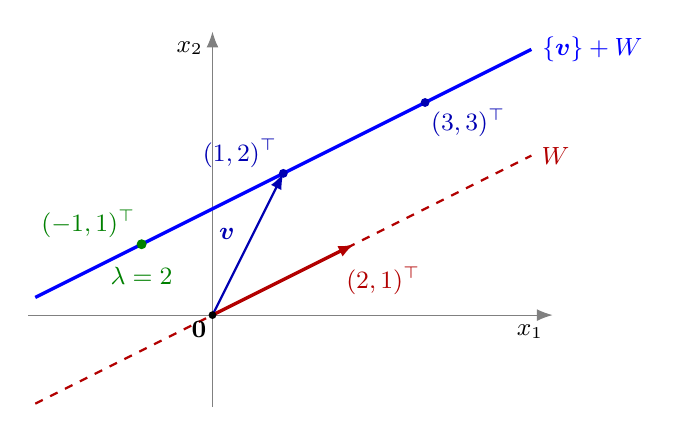
\begin{tikzpicture}[font=\small, >={Latex[length=2mm]}, x=0.9cm, y=0.9cm]
  % axes
  \draw[->, gray] (-2.6,0) -- (4.8,0) node[below left, black] {$x_1$};
  \draw[->, gray] (0,-1.3) -- (0,4.0) node[below left, black] {$x_2$};
  % direction space W through the origin
  \draw[red!70!black, thick, dashed] (-2.5,-1.25) -- (4.5,2.25)
    node[right] {$W$};
  % the affine line {v} + W
  \draw[blue, very thick] (-2.5,0.25) -- (4.5,3.75)
    node[right] {$\{\boldsymbol{v}\}+W$};
  % base point v and direction (2,1)^T
  \draw[->, blue!70!black, thick] (0,0) -- (1,2);
  \node[blue!70!black, anchor=east] at (0.45,1.15) {$\boldsymbol{v}$};
  \draw[->, red!70!black, very thick] (0,0) -- (2,1);
  \node[red!70!black, anchor=north west] at (1.75,0.82) {$(2,1)^{\top}$};
  % points on the line
  \fill[blue!70!black] (1,2) circle (1.6pt) node[above left, inner sep=2pt] {$(1,2)^{\top}$};
  \fill[blue!70!black] (3,3) circle (1.6pt) node[below right, inner sep=2pt] {$(3,3)^{\top}$};
  \fill[green!50!black] (-1,1) circle (1.8pt) node[above left, inner sep=2pt] {$(-1,1)^{\top}$};
  \node[green!50!black, anchor=north] at (-1,0.82) {$\lambda=2$};
  % origin not on the line
  \fill (0,0) circle (1.4pt) node[below left, inner sep=2pt] {$\boldsymbol{0}$};
\end{tikzpicture}
\end{document}
